\chapter{Diagonalización}


Fijemos un $F-$espacio vectorial $V$ de dimensión finita $n$
y una
transformación lineal $T: V \longrightarrow V$ de $V$ en sí mismo.
En el capítulo 
\ref{chapter: representaciones matriciales de transformaciones lineales}
se estudió cómo, escogiendo 
\marginnote{Recuerda que, en la práctica, para hacer cálculos con una
transformación $T:V \longrightarrow V$, es mucho más cómodo usar
representaciones matriciales de esta, es decir, 
pasar del espacio vectorial $\mathcal{L}(V, V)$ al espacio isomorfo
$M_{n \times n}(F)$.}
una base $\beta$ de $V$, podemos definir a la matriz
$[T]_{\beta}^{\beta}$, que guarda la información de $T$ en un arreglo 
de $n^{2}$ elementos del campo $F$. 
Nos interesa ahora no sólo el poder representar
a $T$ con una matriz, también queremos que 
tal representación matricial sea lo más sencilla posible - por ejemplo,
podríamos desear que $[T]_{\beta}^{\beta}$ tenga ``muchas'' entradas nulas,
pues eso reducirá significativamente las operaciones a realizar - y, aún más importante, 
reducirá los errores numéricos en el proceso de cálculo. 
Una situación ideal sería poder encontrar $\beta$ tal que 
$[T]_{\beta}^{\beta}$ sea \textit{diagonal}, digamos, 
\begin{equation}
	\label{eq: repr diagonal, 1}
	[T]_{\beta}^{\beta} = Diag(\lambda_{1}, \ldots , \lambda_{n})
	= \begin{pmatrix}
		\lambda_{1} & 0 & \cdots & 0 \\
		0 & \lambda_{2} & \cdots & 0 \\
		\cdots & \cdots & \cdots & \cdots \\
		0 & 0 & \cdots & \lambda_{n}
	\end{pmatrix}
	,
\end{equation}
\begin{itemize}
	\item En este caso, 
	el rango de $T$ - o sea, la dimensión del espacio 
	vectorial $T(V)$ - es igual a la cantidad de entradas no cero
	de $[T]_{\beta}^{\beta}$ (c.f. Proposición 
	\ref{prop: rango de transf lineal es rango de repr matr cualquiera}).
	\item 
	Representaciones matriciales diagonales simplifican la 
	evaluación de $T$ a vectores del espacio; si $x \in V$ y
	$[x]_{\beta} = (x_{1}, \ldots , x_{n})$, entonces
	\[
	[T(x)]_{\beta} = Diag(\lambda_{1}, \ldots , \lambda_{n}) \cdot 
	\begin{pmatrix}
		x_{1} \\
		x_{2} \\
		\vdots \\
		x_{n} 
	\end{pmatrix}
	= \begin{pmatrix}
		x_{1}\lambda_{1} \\
		x_{2} \lambda_{2} \\
		\vdots \\
		x_{n} \lambda_{n}
	\end{pmatrix}.
	\]
	En general, si $m \geq 1$ y por $T^{m}$ 
	denotamos a la transformación lineal que
	resulta de componer a $T$ consigo mismo $m$ veces,
	es fácil demostrar (por ejemplo, por inducción matemática), que 
	\[
	[T^{m}(x)] = 
	\begin{pmatrix}
		x_{1}\lambda_{1}^{m} \\
		x_{2} \lambda_{2}^{m} \\
		\vdots \\
		x_{n} \lambda_{n}^{m}
	\end{pmatrix}.
	\]
	\begin{marginfigure}
		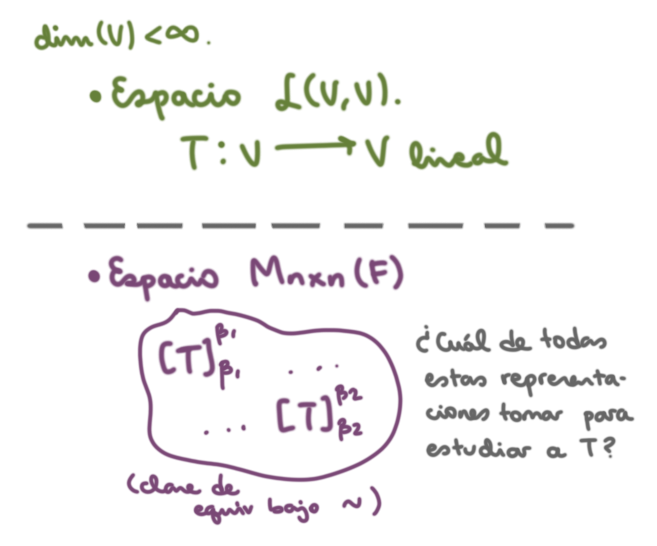
\includegraphics[scale=1.7]{24} 
	\end{marginfigure}
	\item El determinante de la matriz 
	\eqref{eq: repr diagonal, 1} (que después usaremos para definir el
	determinante de la transformación $T$) es simplemente el producto
	de sus entradas diagonales;
	\[
	det(Diag(\lambda_{1}, \ldots , \lambda_{n}))
	= \Pi_{j = 1}^{n} \lambda_{j}.
	\]
\end{itemize}

La pregunta ahora es qué transformaciones lineales
$T: V \longrightarrow V$ admiten una representación matricial diagonal. 
En este último capítulo, daremos condiciones necesarias y suficientes 
para la existencia de tal representación, que será usada para
\hlpink{termina. Procesos de Markov, aplicación a Probabilidad.}


\section{Operadores lineales diagonalizables}
Fijemos a un $F$-espacio vectorial $V$ con $dim(V) < \infty$.
\begin{defi}
Toda transformación lineal $T: V \longrightarrow V$
de un $F-$espacio vectorial $V$ en sí mismo es llamada un
\textbf{operador lineal} sobre $V$.
\end{defi}
 

\begin{defi}
Una matriz $D = (d_{ij})
\in M_{n \times n}(F)$ se dice \textbf{diagonal} si sólo
sus entradas $d_{ii}$ pueden no ser cero.
\end{defi}

Recuerda que, dadas $T: V \longrightarrow V$ lineal y una base
$\beta \subseteq V$, la clase de equivalencia de la matriz
$[T]_{\beta}^{\beta}$ 
bajo la relación ``ser similar a''
(c.f. Definición \ref{def: matrices similares})
consta \textit{exactamente} de otras representaciones
matriciales $[T]_{\beta'}^{\beta'}$ de la misma transformación 
lineal $T$ 
(c.f. Teorema 
\ref{teo: similar a repr matricial de T sii tambien es repr matr de T}).
Nos gustaría saber cuándo $T$ es tal que una de esas representaciones
matriciales es diagonal.

\begin{defi}
	\label{def: operador diagonalizable}
Se dice que un operador lineal $T: V \longrightarrow V$ sobre
un $F-$espacio vectorial finito dimensional $V$ es
\textbf{diagonalizable} si existe una base $\beta$ de $V$
tal que $[T]_{\beta}^{\beta}$ es una matriz diagonal.
\textbf{Diagonalizar un operador $T$} se refiere a encontrar
(cuando sea posible) una base $\beta$ de $V$ tal que
$D:= [T]_{\beta}^{\beta}$ es diagonal.
\end{defi}
\marginnote{Cuidado: no confundas los conceptos de ``matriz diagonal''
	y ``matriz diagonalizable''.}
Tenemos una definición dual a la \ref{def: operador diagonalizable}
para matrices:
\begin{defi}
	\label{def: matriz diagonalizable}
Una matriz cuadrada $A$ es \textbf{diagonalizable} si $A$
es similar a una matriz diagonal. 
\textbf{Diagonalizar una matriz $A$} se refiere a encontrar
(cuando sea posible) una matriz invertible $Q$ tal que 
$D = Q^{-1} A Q$.
\end{defi}

\begin{figure}[H]
	\sidecaption{
	Los dos conceptos de diagonalización en los espacios isomorfos
	$\mathcal{L}(V, V)$ y $M_{n \times n}(F)$.
	}
	\centering
	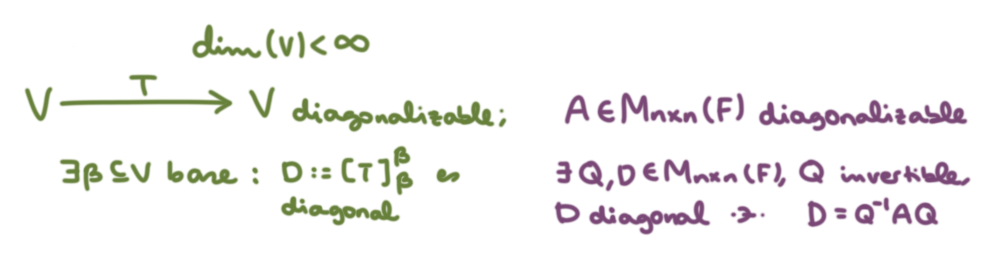
\includegraphics[scale = 3]{26} 
\end{figure}	


Pensando siempre en establecer una conección entre
las definiciones hechas en el espacio
$\mathcal{L}(V, V)$ y el espacio $M_{n \times n}(F)$,
relacionamos las dos nociones de ``ser diagonalizable'' a continuación.
\begin{prop}
Sean $V$ un $F-$espacio vectorial finito dimensional, $T: V \longrightarrow V$
un operador lineal en $V$. Las siguientes son equivalentes:
\begin{itemize}
	\item[$a)$] $T$ es un operador diagonalizable
	\item[$b)$] Existe una base $\beta$ de $V$ tal que la matriz
	$[T]_{\beta}^{\beta}$ es diagonalizable 
	\item[$c)$] Para toda base $\gamma$ de $V$, la representación
	matricial $[T]_{\gamma}^{\gamma}$ es diagonalizable.
\end{itemize}
\end{prop}

\begin{figure}[H]
\centering
	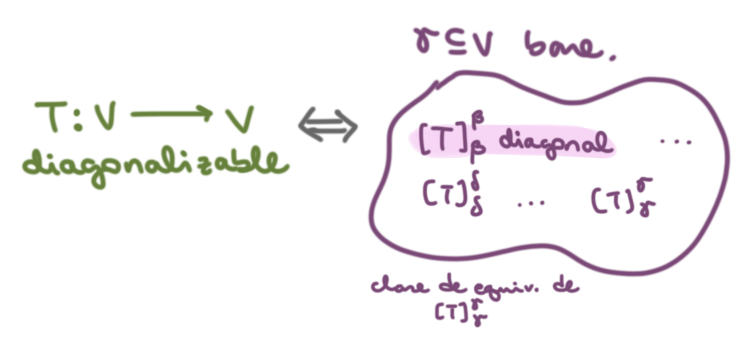
\includegraphics[scale=3.2]{25}
 \end{figure}
\noindent
\textbf{Demostración.}
\marginnote{Recuerda que con $\sim$ denotamos a la relación de equivalencia
``ser similar a''.}
\begin{itemize}
	\item[$a) \Rightarrow b) )$] Sea $\beta \subseteq V$ base tal que 
	$A = [T]_{\beta}^{\beta}$ es una matriz diagonal. Como 
	$A$ es trivialmente similar a sí misma, $\beta$ es una base que
	satisface el inciso $b)$.
	\item[$b) \Rightarrow c) )$] Sea $\beta$ una base de $V$ tal que
	la matriz $[T]_{\beta}^{\beta}$ es diagonalizable; esto significa
	que existe $D$ matriz diagonal tal que
	\[
	[T]_{\beta}^{\beta} \sim D.
	\]
	Si $\gamma$ es cualquier otra base de $V$, entonces, por el Teorema
	\ref{teo: similar a repr matricial de T sii tambien es repr matr de T},
	también se tiene
	\[
	[T]_{\gamma}^{\gamma} \sim [T]_{\beta}^{\beta}.
	\]
	De la transitividad de $\sim$ se deduce que 
	$[T]_{\gamma}^{\gamma} \sim D$, o sea, que $[T]_{\gamma}^{\gamma}$
	es diagonalizable.
	\item[$c) \Rightarrow a) )$] Sea $\gamma$ una base cualquiera de $V$.
	Por hipóteis, $[T]_{\gamma}^{\gamma}$ es diagonalizable, es decir,
	existe $D$ diagonal tal que $[T]_{\gamma}^{\gamma} \sim D$. Según
	el Teorema 
	\ref{teo: similar a repr matricial de T sii tambien es repr matr de T},
	esto implica que la matriz $D$ también es una representación matricial
	de $T$ respecto a una misma base del espacio. 
	Así, $T$ es diagonalizable.
\end{itemize}
\QEDB
\vspace{0.2cm}

\begin{cor} La matriz
$A \in M_{n \times n}(F)$ es diagonalizable si y sólo si 
el operador
$L_{A}: F^{n} \longrightarrow F^{n}$ es diagonalizable.
\end{cor}
\noindent
\textbf{Demostración.}
Recuerda que si 
$\beta$ es la base canónica de $F^{n}$ entonces 
$[L_{A}]_{\beta}^{\beta} = A$, luego, 
\begin{itemize}
	\item si $A$ es diagonalizable, es decir, si 
	existe $D$ diagonal con $D = Q^{-1} A Q$ para alguna matriz
	invertible $Q$,
como $D$ es similar a $A$, por el Teorema
\ref{teo: similar a repr matricial de T sii tambien es repr matr de T}
existe otra base $\gamma \in F^{n}$ tal que
$D = [L_{A}]_{\gamma}^{\gamma}$, luego, $L_{A}$ es un operador
diagonalizable;
\marginnote{En este sentido, 
diagonalizar a la
matriz $A$ es lo mismo que diagonalizar al operador $L_{A}$.}
	\item recíprocamente, si $L_{A}: F^{n} \longrightarrow F^{n}$ es un operador
diagonalizable, entonces existe $\gamma$ base de $F^{n}$
tal que $D := [L_{A}]_{\gamma}^{\gamma}$ es diagonal. Como $A$
también es una representación matricial de $L_{A}$, $D$ y 
$A$ son similares, de hecho,
\[
D = Q^{-1} A Q, \hspace{0.2cm} \textit{ donde }
Q = [Id]_{\gamma}^{\beta},
\]
luego, $A$ es una matriz diagonalizable.
\end{itemize}
\QEDB
\vspace{0.2cm}


Definidos ya los conceptos que deseamos estudiar, 
encaremos la pregunta
con la que iniciamos el capítulo: ¿qué debe cumplir un operador 
$T: V \longrightarrow V$ para que exista una base
$\beta \subseteq V$ tal que $[T]_{\beta}^{\beta}$ sea diagonal?
Observa que
\begin{itemize}
	\item si tal $\beta = \{ v_{1}, \ldots, v_{n} \}$ existe, si 
	\begin{equation}
		\label{eq: diagonal de T}
		[T]_{\beta}^{\beta} = \begin{pmatrix}
	\lambda_{1} & 0 & 0 & \ldots & 0 \\
	0 & \lambda_{2} & 0 & \ldots & 0 \\
	0 & 0 & \lambda_{3} & \ldots & 0 \\
	\ldots & \ldots & \ldots & \ldots & \ldots \\
	0 & 0 & 0 & \ldots & \lambda_{n} 
	\end{pmatrix},
	\end{equation}
	podemos usar esta representación para saber cómo actua $T$ en la
	base $\beta$, pues, 
	\[
	\forall 1 \leq j \leq n: \hspace{0.2cm}
	T(v_{j}) = 0 v_{1} + \ldots + \lambda_{j} v_{j} + \ldots + 0 v_{n},
	\]
	o sea, 
	\begin{equation}
	\label{eq: T actuando en base de eigenvectores}
	\forall 1 \leq j \leq n: \hspace{0.2cm}
	T(v_{j}) = \lambda_{j} v_{j}.
	\end{equation}
	\item Recíprocamente, si una base satisface la condición
	\eqref{eq: T actuando en base de eigenvectores}, entonces
	claro que su representación matricial respecto a esa base
	es diagonal, de hecho, es la matriz 
	\eqref{eq: diagonal de T}.
\end{itemize}
Queda demostrada así la siguiente
\begin{prop}
	\label{prop: condicion sii de operador diagonalizable}
	Sean $V$ un $F-$espacio vectorial finito dimensional,
	$T: V \longrightarrow V$ un operador sobre este. $T$
	es diagonalizable si y sólo si existe una base 
	$\beta = \{ v_{j}  | \hspace{0.2cm} 1 \leq j \leq n \}$ de $V$
	para la que existan escalares $\lambda_{j}$, $1 \leq j \leq n$
	tales que
	\[
	\forall 1 \leq j \leq n: \hspace{0.2cm}
	T(v_{j}) = \lambda_{j}v_{j}.
	\]
\end{prop}
Esta caracterización de diagonalizabilidad motiva las siguientes
definiciones.
\begin{defi}
	\label{def: vector y valor propio}
	\marginnote{Algunos autores usan los nombres ``eigenvector'' y 
	``eigenvalue''.}
	Sea $T: V \longrightarrow V$ un operador lineal.	
	Un vector $v \in V - \{ 0 \}$ es un \textbf{autovector} de 
	$T$ si existe $\lambda \in V$ tal que 
	$T(v) = \lambda v$ (i.e. $v$ y su imagen bajo $T$ son paralelos).
	Al escalar $\lambda$ se le llama el \textbf{autovalor} 
	asociado a $v$.
	
	Sea $A \in M_{n \times n}(F)$ una matriz cuadrada. Un 
	vector $v \in F^{n} - \{ 0 \}$ es un \textbf{autovector}
	de $A$ si es un vector propio del operador $L_{A}$.
\end{defi}

Puesto que 
\[
\forall \lambda \in F: \hspace{0.2cm}
T(0) = 0 = \lambda 0,
\]
se excluye al vector cero de la definición de autovector.


\marginnote{Así, diagonalizar un operador consiste en encontrar una base
del espacio que conste de vectores propios de este.}
Con esta nueva terminología, la Proposición 
\ref{prop: condicion sii de operador diagonalizable} se reformula
como ``un operador $T:V \longrightarrow V$ es diagonalizable si y sólo si
existe una base de $V$ compuesta de vectores propios de $T$''.


\begin{defi}
	\label{def: espectro de operador y espacios E lambda}
Sea $T: V \longrightarrow V$ operador.
\begin{itemize}
	\item Denotaremos al conjunto de valores propios de $T$ por
	\begin{equation}
	\label{eq: espectro de T}
		spec(T) := \{ \lambda \in F  | \hspace{0.2cm}  
		\exists v \in V-\{ 0 \}: \hspace{0.1cm} T(v) = \lambda v
		\}.
	\end{equation}
	A este se la llamará el \textbf{espectro de $T$}.
	\item Para cada $\lambda \in F$, denotaremos
	al conjunto de vectores de $V$ que cumplen que 
	$T(v) = \lambda v$, o sea,
	\begin{equation}
		\label{eq: espacios de vect propios de T}
		E_{\lambda} := \{ v \in V  | \hspace{0.2cm} T(v) = \lambda v \}.
	\end{equation}
\end{itemize}
\end{defi}

\hlgray{Ejercicio:} Demuestra que, para cada $\lambda \in F$,
$E_{\lambda}$ es un subespacio de $V$.

\hlgray{Ejercicio:} Demuestra que un vector propio tiene un y sólo
un valor propio. En otras palabras, demuestra que son equivalentes 
las siguientes proposiciones: para $\lambda, \lambda' \in F$,
\begin{itemize}
	\item $\lambda \neq \lambda'$.
	\item $E_{\lambda} \cap E_{\lambda'} = \{0\}$.
	\item $E_{\lambda} \oplus E_{\lambda'}$.
\end{itemize}

\begin{obs}
	Para todo $\lambda \in F$, 
	$\lambda \in spec(T)$ si y sólo si $\{ 0 \} \subsetneq E_{\lambda}$.
\end{obs}

\begin{ejem} 
\label{ejem: operadores diagn y no diagn}	
(De operadores en $\IR^{2}$, uno de ellos diagonalizable
y el otro no).
\begin{itemize}
	\item Considere a un ángulo $\theta \in [0, 2 \pi[$, y sea
	$R_{\theta}$ la rotación respecto al origen de $\theta$
	radianes \TODO{referencia}. ¿Es diagonalizable $R_{\theta}$?
	Determina $Spec(R_{\theta})$.
	
	\item Considere a la matriz
	\[
	A = \begin{pmatrix}
	1 & 3 \\ 4 & 2
	\end{pmatrix}.
	\]
	Puede comprobar que 
	\[
	v_{1} = \begin{pmatrix}
	1 \\ -1
	\end{pmatrix}, \hspace{0.2cm}
	v_{2} = \begin{pmatrix}
	3 \\ 4
	\end{pmatrix}
	\]
	son ambos vectores propios de $A$, con respectivos valores propios
	$-2$ y $5$. Entonces, si $\beta = \{ v_{1}, v_{2} \}$, 
	\[
	[L_{A}]_{\beta}^{\beta} = \begin{pmatrix}
	-2 & 0 \\ 0 & 5
	\end{pmatrix}.
	\]
\end{itemize}
\end{ejem}

\hlgray{Ejercicio:} Demuestra que $Spec(Id_{V}) = \{1\}$, y que, en 
este caso, $E_{1} = V$.

\begin{ejem}
	(De los autovalores de un operador en un espacio infinito dimensional).
	
	Considere al espacio $\IR^{\IN}$ de sucesiones reales. En este espacio,
	sea $L: \IR^{\IN} \longrightarrow \IR^{\IN}$ el operador 
	left-shift:
	\[
	L((x_{0}, x_{1}, x_{2}, \ldots  )) = (
	x_{1}, x_{2}, \ldots
	).
	\]
	Si a partir de $k \in \IR$ definimos a la sucesión
	\[
	\hat{k} = (1, k, k^{2}, k^{3}, \ldots),
	\]
	tenemos que 
	\[
	L(\hat{k}) = (k, k^{2}, k^{3}, \ldots) = 
	k \hat{k}.
	\]
	Así, todo número real es autovalor de $L$.
\end{ejem}



\begin{ejem}
Observe que si $T: V \longrightarrow V$ no es inyectivo, entonces
tiene una infinidad de vectores propios con valor propio cero.
En efecto, el que $T$ no sea inyectivo significa que 
$\{ 0 \} \neq Ker(T)$; sea pues $v \in Ker(T)- \{ 0 \}$.
\[
T(v) = 0_{V} = 0_{F} \cdot v.
\]
De hecho, 
\[
\forall a \in F: \hspace{0.2cm} 
T(av) = a T(v) = a \cdot 0_{V} = 0_{V}.
\]
Así, todo elemento de $span(\{v\})$
es un vector propio con valor propio cero.
\end{ejem}

En el Ejemplo \ref{ejem: operadores diagn y no diagn}	
se te dieron sugerencias de autovectores de 
la matriz $A$, ¿cómo encontramos (de existir) los autovalores y autovectores
de un operador?

El siguiente resultado es extremadamente útil en la práctica,
pues nos permite pasar de un proceso de diagonalización en un
espacio vectorial finito dimensional cualquiera $V$
(en el que puede ser difícil trabajar directamente) a un proceso
de diagonalización en el espacio $M_{n \times n} (F)$ 
(espacio en el que nunca tenemos problemas para realizar los
cálculos correspondientes). 
\marginnote{Una aplicación importante de esta
Proposición se muestra en el Ejemplo \TODO{referencia}.}
\begin{prop}
	\label{prop: autovectores de T sii de su analogo en matrices}
$T: V \longrightarrow V$ operador, $\beta \subseteq V$ base,
$A = [T]_{\beta}^{\beta}$ su representación matricial respecto a $\beta$.
$T$ y $A$ tienen los mismos valores propios; además,
$v \in V$ es vector propio de $T$ si y sólo si $x = [v]_{\beta}$
es vector propio de $L_{A}$. 
\end{prop}
\begin{center}
\begin{tikzpicture}[x=0.75pt,y=0.75pt,yscale=-1,xscale=1]
%uncomment if require: \path (0,235); %set diagram left start at 0, and has height of 235


% Text Node
\draw (259.06,70.66) node    {$V$};
% Text Node
\draw (123.37,70.66) node  [color={rgb, 255:red, 0; green, 0; blue, 0 }  ,opacity=1 ]  {$V$};
% Text Node
\draw (259.06,161.19) node    {$F^{m}$};
% Text Node
\draw (123.37,161.19) node    {$F^{n}$};
% Text Node
\draw (190.29,174.51) node    {$L_{A}$};
% Text Node
\draw (102.29,111.51) node  [font=\footnotesize,color={rgb, 255:red, 0; green, 0; blue, 0 }  ,opacity=1 ]  {$[ \cdotp ]_{\beta }$};
% Text Node
\draw (282.78,111.51) node  [font=\footnotesize,color={rgb, 255:red, 0; green, 0; blue, 0 }  ,opacity=1 ]  {$[ \cdotp ]_{\beta }$};
% Text Node
\draw (190.6,60.03) node    {$T$};
% Text Node
\draw (104.6,70.03) node  [font=\footnotesize,color={rgb, 255:red, 65; green, 117; blue, 5 }  ,opacity=1 ]  {$v\in $};
% Text Node
\draw (81.6,163.03) node  [font=\footnotesize,color={rgb, 255:red, 129; green, 22; blue, 149 }  ,opacity=1 ]  {$x=\ [ v]_{\beta } \in $};
% Connection
\draw    (132.87,70.66) -- (247.56,70.66) ;
\draw [shift={(249.56,70.66)}, rotate = 180] [color={rgb, 255:red, 0; green, 0; blue, 0 }  ][line width=0.75]    (10.93,-3.29) .. controls (6.95,-1.4) and (3.31,-0.3) .. (0,0) .. controls (3.31,0.3) and (6.95,1.4) .. (10.93,3.29)   ;
% Connection
\draw    (135.87,161.19) -- (243.06,161.19) ;
\draw [shift={(245.06,161.19)}, rotate = 180] [color={rgb, 255:red, 0; green, 0; blue, 0 }  ][line width=0.75]    (10.93,-3.29) .. controls (6.95,-1.4) and (3.31,-0.3) .. (0,0) .. controls (3.31,0.3) and (6.95,1.4) .. (10.93,3.29)   ;
% Connection
\draw [color={rgb, 255:red, 0; green, 0; blue, 0 }  ,draw opacity=1 ]   (123.37,82.66) -- (123.37,146.69) ;
\draw [shift={(123.37,148.69)}, rotate = 270] [color={rgb, 255:red, 0; green, 0; blue, 0 }  ,draw opacity=1 ][line width=0.75]    (10.93,-3.29) .. controls (6.95,-1.4) and (3.31,-0.3) .. (0,0) .. controls (3.31,0.3) and (6.95,1.4) .. (10.93,3.29)   ;
% Connection
\draw [color={rgb, 255:red, 0; green, 0; blue, 0 }  ,draw opacity=1 ]   (259.06,82.66) -- (259.06,146.69) ;
\draw [shift={(259.06,148.69)}, rotate = 270] [color={rgb, 255:red, 0; green, 0; blue, 0 }  ,draw opacity=1 ][line width=0.75]    (10.93,-3.29) .. controls (6.95,-1.4) and (3.31,-0.3) .. (0,0) .. controls (3.31,0.3) and (6.95,1.4) .. (10.93,3.29)   ;
\end{tikzpicture}
\end{center}
\marginnote{
La Proposición 
\ref{prop: autovectores de T sii de su analogo en matrices}
nos permite cambiar la pregunta ¿es $x$ un autovector de 
$T$? por ¿es $[x]_{\beta}$ un autovector de $L_{A3}$?}
\noindent
\textbf{Demostración.}
En efecto, dado $v \in V$, si $x = [v]_{\beta}$, entonces
\begin{align*}
T(v) = \lambda v & \textit{ sii } [T(v)]_{\beta} = [\lambda v]_{\beta} \\
& \textit{ sii } [T]_{\beta}^{\beta} [v]_{\beta} = \lambda [v]_{\beta} \\
& \textit{ sii } A x = \lambda x \\
& \textit{ sii } L_{A}(x) = \lambda x.
\end{align*}
\QEDB
\vspace{0.2cm}


\section{El determinante de un operador y su polinomio característico}

Sea $T: V \longrightarrow V$ un operador. Observa que,
dado $\lambda \in F$ cualquiera,

\begin{align*}
T(v) = \lambda v & \textit{ sii }  T(v) = \lambda Id(v) \\
& \textit{ sii }  (T - \lambda Id )( v ) = 0 \\
& \textit{ sii } v \in Ker(T - \lambda Id),
\end{align*}
luego, $\lambda$ es un autovalor de $T$ si y sólo si
en el Kernel del operador en $V$
$$ U_{\lambda} := T- \lambda Id $$ hay vectores no cero -
es decir, si y sólo si 
$U_{\lambda}$ no es inyectiva
(c.f
Proposición
\ref{prop: caracterizacion de inyectividad}).
Recordando las notaciones introducidas en 
la Definición \ref{def: espectro de operador y espacios E lambda},
tenemos que
\marginnote{Por \eqref{eq: espacios de autovectores como Kernel}
identificamos a los espacios de autovalores $E_{\lambda}$ para
$\lambda \in spec(T)$ como subespacios de $V$.}
\begin{equation}
	\label{eq: espacios de autovectores como Kernel}
	\forall \lambda \in F: \hspace{0.2cm}
	E_{\lambda} = Ker(T- \lambda ID) = Ker(U_{\lambda}).
\end{equation}
Resumimos esto en la siguiente
\begin{obs}
	Para todo $\lambda \in F$, 
	$\lambda \in spec(T)$ si y sólo si
	$\{ 0 \} \subsetneq Ker(U_{\lambda})$.
\end{obs}
Este razonamiento nos permite identificar fácilmente los
autovalores de $T$ - y, a partir de ellos, a los autovectores de $T$.
\begin{prop}
	\label{prop: lambda autovalor sii det cero}
Sea $T: V \longrightarrow V$ un operador lineal en un espacio
$V$ finito dimensional. Sea $A = [T]_{\beta}^{\beta}$ una representación
matricial de $T$. 
Las siguientes son equivalentes:
\begin{itemize}
	\item $\lambda \in F$ es un autovalor de $T$.
	\item $det(A - \lambda I_{n}) = 0$.
\end{itemize}
\end{prop}
\noindent
\textbf{Demostración.}
Por lo discutido arriba, 
si $U_{\lambda} := T - \lambda Id: V \longrightarrow V$, entonces
$\lambda$ es un autovalor de $T$ si y sólo
si $U_{\lambda}$ no es inyectiva; como $V$ es finito dimensional,
esto equivale a que $U_{\lambda}$ no sea invertible 
(c.f. Proposición \ref{teo: inyectiva sii supra sii biyect en dim finita}); 
esto, según el Teorema \TODO{cita} equivale a que 
su representación matricial 
\[
[U_{\lambda}]_{\beta}^{\beta} = [T - \lambda Id]_{\beta}^{\beta}
= A - \lambda I_{n}
\]
no sea invertible, lo que a su vez equivale a que 
el determinante de $A - \lambda I_{n}$ sea cero.
\QEDB
\vspace{0.2cm}


\begin{lema}
	\label{lema: determinante de repr de T es invariante a la base tomada}
	Sean $V$ finito dimensional, $\beta, \beta' \subseteq V$ bases,
	$T: V \longrightarrow V$ un operador en $V$.
	Se tiene que
	\[
	det([T]_{\beta}^{\beta}) = det([T]_{\beta'}^{\beta'}).
	\]
\end{lema}
\marginnote{Recuerda que, si $A, B \in M_{n \times n}(F)$, entonces
$det(AB) = det(A) \cdot det(B)$. De esto se deduce además que, si 
$A$ es invertible, entonces $det(A^{-1}) = det(A)^{-1}$.}
\noindent
\textbf{Demostración.}
En efecto, haciendo
$A = [T]_{\beta}^{\beta}$ y $B = [T]_{\beta'}^{\beta'}$,
sólo note que si $Q$ es la matriz invertible $[Id_{n}]_{\beta'}^{\beta}$,
entonces
\begin{align*}
det(B) = & det(Q^{-1} A Q) = det(Q^{-1}) det(A) det(Q) \\
= & det(Q)^{-1} det(A) det(Q) = det(A).
\end{align*}

\QEDB
\vspace{0.2cm}

Lo demostrado en el Lema
\ref{lema: determinante de repr de T es invariante a la base tomada}
hace legítima la siguiente
\begin{defi}
	\label{def: determinante de un operador}
	Dado $T: V \longrightarrow V$ en un espacio finito dimensional $V$,
	definimos su \textbf{determinante} como 
	\[
	det(T) = det([T]_{\beta}^{\beta}), \hspace{0.2cm}
	\beta \subseteq V \textit{ base.}
	\]
\end{defi}
\noindent

\begin{lema}
Sea $T: V \longrightarrow V$ un operador. Si $\lambda$ es un escalar,
$\beta$ es una base de $V$ y $A = [T]_{\beta}^{\beta}$, entonces
\begin{equation}
	\label{eq: det T - lambda I det A - lambda I}
	det(T - \lambda Id) = det(A - \lambda I).
\end{equation}
\end{lema}
\noindent
\textbf{Demostración.}
Recordando que $[Id]_{\beta}^{\beta} = I_{n}$ y que la representación
matricial de una suma es la suma de las representaciones, tenemos que
\[
det(T - \lambda Id) = det([T - \lambda Id]_{\beta}^{\beta}) 
= det([T]_{\beta}^{\beta} - \lambda[Id]_{\beta}^{\beta})
= det(A - \lambda I_{n}).
\]

\QEDB
\vspace{0.2cm}


Podemos reformular a la Proposición 
\ref{prop: lambda autovalor sii det cero} como sigue.
\begin{cor}
Dado $T: V \longrightarrow V$ operador en 
un $F-$espacio finito dimensional $V$,
$\lambda \in F$ es un autovalor de $T$ si y sólo si 
$det(U_{\lambda}) = 0$, donde $U_{\lambda} = T - \lambda Id$.
\end{cor}


\begin{defi}
	\label{def: polinomio caracteristico}
	Sea $T: V \longrightarrow V$ un operador lineal en un espacio
	finito dimnesional $V$. 
	El polinomio
	\[
	p(\lambda) := det(T - \lambda Id)
	\]
	es llamado el \textbf{polinomio característico de $T$}.
\end{defi}

\begin{prop}
	\label{prop: propiedades del pol caracteristico}
	Sean $T : V \longrightarrow V$ operador, con $dim(V) = n$, 
	$p(\lambda)$ su polinomio característico.
	\begin{itemize}
		\item Las raíces de $p(\lambda)$ son 
		son exactamente los autovalores de $T$, o sea, 
		\[
		\forall \lambda \in F: \hspace{0.2cm}
		\lambda \in Spec(T) \hspace{0.2cm}
		\Leftrightarrow \hspace{0.2cm} p(\lambda) = 0.
		\]
		\item El grado de $p(\lambda)$ es $n$.
		\item Si $T$ es diagonalizable, entonces $p$ se factoriza como
		un producto de $n$ polinomios de grado $1$ no necesariamente distintos
		entre sí.
	\end{itemize}
\end{prop}
\marginnote{Según la Proposición 
\ref{prop: propiedades del pol caracteristico}, 
si el polinomio característico de un operador $T$ no se descompone
como producto de polinomios de grado $1$, entonces $T$ no es diagonalizable.}
\textbf{Demostración.}
Si $\beta$ es base de $V$ tal que 
$[T]_{\beta}^{\beta} = Diag(\lambda_{1}, \ldots , \lambda_{n})$,
entonces 
\[
p(\lambda) = det(T- \lambda I) = det
\begin{pmatrix}
	\lambda_{1} - \lambda & 0 & \cdots & 0 \\
	0 & \lambda_{1} - \lambda & \cdots & 0 \\
	\cdots & \cdots & \cdots & \cdots \\
	0 & 0 & \cdots & \lambda_{n} - \lambda
\end{pmatrix}
= \Pi_{j=1}^{n} (\lambda_{j} - \lambda).
\]

\QEDB
\vspace{0.2cm}

Mostremos con un ejemplo que la suficiencia en el tercer
punto de la Proposición 
\ref{prop: propiedades del pol caracteristico}
no se tiene; aún cuando el polinomio
característico de $T: V \longrightarrow V$ se pueda factorizar
como producto de polinomios de grado uno, puede ser que $T$
no sea diagonalizable.

\begin{ejem}
	\label{ej: de un operador con polinomio caract factorizable en pol de grado uno que no es diagonalizable}
	Sea $T: P_{2}(\IR) \longrightarrow P_{2}(\IR)$ el operador 
	derivación. Si consideramos a la base
	$\beta = \{ 1, x, x^{2} \}$ del espacio de polinomios reales
	de grado a lo más $2$, se calcula que 
	\[
	[T]_{\beta}^{\beta} = \begin{pmatrix}
		0 & 1 & 0 \\
		0 & 0 & 2 \\
		0 & 0 & 0
	\end{pmatrix}.
	\]
	A partir de esta representación matricial, calculamos al
	polinomio característico de $p$;
	\[
	p(\lambda) = det 
	\begin{pmatrix}
		-\lambda & 1 & 0 \\
		0 &-\lambda & 2 \\
		0 & 0 & - \lambda
	\end{pmatrix} = - \lambda^{3}.
	\]
	Así, $Spec(T) = \{0\}$, o sea, $T$ sólo tiene autovalores de 
	autovector cero.
	\begin{align*}
		E_{0} = & \{f \in P_{2}(\IR) : \hspace{0.2cm} f' = 0 \} \\
		= & \{f \in P_{2}(\IR) : \hspace{0.2cm} \textit{ f es un polinomio constante} \}.
	\end{align*}
	Claro que $dim(E_{0}) = 1$, luego, es imposible formar una base 
	del espacio $P_{2}(\IR)$ - que tiene dimensión $3$ - a partir de
	autovectores de $T$, es decir, $T$ no es diagonalizable, pues 
	no hay ``suficientes'' autovectores de $T $ linealmente independientes.
	$\diamond$
\end{ejem}

\begin{cor}
	Sean $D_{1}, D_{2} \in M_{n \times n}(F)$ matrices cuadradas diagonales, digamos
	\[
	D_{1} = Diag(\lambda_{1}, \cdots , \lambda_{n}), \hspace{0.2cm}
	D_{2} = Diag(\mu_{1}, \cdots , \mu_{n}).
	\]
	Si $D_{1}$ y $D_{2}$ son similares, entonces, salvo permutación, tienen
	las mismas entradas diagonales, es decir, existe
	$\rho : \{1, \ldots , n\} \longrightarrow \{1, \ldots , n\}$
	biyección tal que 
	\[
	\forall 1 \leq j \leq n: \hspace{0.2cm} \lambda_{j} = \mu_{\rho(j)}.
	\]
\end{cor}
\textbf{Demostración.}
Consideremos al operador
$T = L_{D_{1}}$ en $F^{n}$.
Si $\beta$ es la base canónica de $F^{n}$, 
\begin{equation}
	\label{eq: cor matrices similares diagonales, 1}
	D_{1} = [T]_{\beta}^{\beta}.
\end{equation}
Por hipótesis, 
$D_{1} \sim D_{2}$, luego, según el Teorema
\ref{teo: similar a repr matricial de T sii tambien es repr matr de T},
existe $\gamma$ base de $V$ tal que 
\begin{equation}
	\label{eq: cor matrices similares diagonales, 2}
	D_{2} = [T]_{\gamma}^{\gamma}.
\end{equation}
Podemos usar estas dos representaciones matriciales para calcular
el polinomio característico de $T$; 
\[
p(\lambda) = det \begin{pmatrix}
	\lambda_{1} - \lambda & 0 & 0 & \cdots & 0 \\
	0 & \lambda_{2} - \lambda &0 & \cdots & 0 \\
	\cdots & \cdots & \cdots & \cdots & \cdots \\
	0 & 0 & 0 & \cdots & \lambda_{n} - \lambda
\end{pmatrix} = \Pi_{j=1}^{n} (\lambda_{j} - \lambda);
\]
\[
p(\lambda) = det \begin{pmatrix}
	\mu_{1} - \lambda & 0 & 0 & \cdots & 0 \\
	0 & \mu_{2} - \lambda &0 & \cdots & 0 \\
	\cdots & \cdots & \cdots & \cdots & \cdots \\
	0 & 0 & 0 & \cdots & \mu_{n} - \lambda
\end{pmatrix} = \Pi_{j=1}^{n} (\mu_{j} - \lambda);
\]
o sea, 
\begin{equation}
	\label{eq: cor matrices similares diagonales, 3}
	\Pi_{j=1}^{n} (\lambda_{j} - \lambda) = 
	\Pi_{j=1}^{n} (\mu_{j} - \lambda) 
	\hspace{1cm} (\textit{ecuación en el dominio entero } F[\lambda]).
\end{equation}
\marginnote{Nota que la ecuación análoga a 
\eqref{eq: cor matrices similares diagonales, 3} en el campo $F$
sería
$$\Pi_{j=1}^{n} \lambda_{j} = \Pi_{j=1}^{n} \mu_{j},$$
y de esta \textbf{no} se puede deducir de inmediato que 
las $\lambda_{j}$ son las $\mu_{j}$ permutadas, pues no necesariamente
son primos en $F$. Este problema se arregla si consideramos, como 
en nuestra demostración, a los irreducibles $(\lambda - \lambda_{j})$
en $F[\lambda]$.
}
Por ser $F$ campo, los polinomios de grado uno son irreducibles
(c.f. \cite{Rotman}), luego, \eqref{eq: cor matrices similares diagonales, 3}
implica que los polinomios de grado uno que aparecen en el producto de la 
derecho son, salvo un reordenamiento, exactamente los que aparecen en el 
producto de la izquierda; esto significa que 
las $\lambda_{j}$ son, salvo un reordenamiento, las $\mu_{j}$.
\QEDB
\vspace{0.2cm}

\hlgray{Ejercicio:} Si $T : \IC^{n} \longrightarrow \IC^{n}$
es un operador en el $\IC-$espacio vectorial $\IC^{n}$, demuestra
que $Spec(T) \neq \emptyset$. Contrasta esto con  
el Ejemplo \ref{ejem: operadores diagn y no diagn}.

\begin{defi}
	\label{def: multiplicidad de un autovector}
	Sean $V$ finito dimensional, $T: V \longrightarrow V$ un operador en $V$.
	Si $\lambda_{0} \in F$ es un autovalor de $T$, definimos su \textbf{multiplicidad
	algebráica} como el mayor entero $m \geq 1$ tal que 
	$(\lambda - \lambda_{0})^{m}$ divide al polinomio 
	característico $p(\lambda)$ de $T$.
\end{defi}


Nota que, si $T$ es diagonalizable - 
digamos que $\beta$ es base de $V$ compuesta de autovectores de $T$ -
y si $\lambda_{1} \in Spec(T)$, entonces
la multiplicidad algebráica de $\lambda_{1}$ corresponde a la
cantidad de elementos de $\beta$ que también están en el 
espacio $E_{\lambda_{1}}$. Observaciones de este tipo nos ayudarán
a construir criterios y algoritmos para la diagonalización de operadores.
Antes de seguir desarrollando la teoría, apliquémosla en algunos ejemplos.

\hlgray{Ejercicio: } Fijado $\theta \in [0, 2\pi[$ ángulo - medido en 
radianes - calcula el polinomio característico de la rotación 
$R_{\theta} : \IR^{2} \longrightarrow \IR^{2}$ por $\theta$
radianes, y úsalo para calcular el espectro de $R_{\theta}$.
Compara esto con el ejercicio \TODO{cita}.

\section{Ejemplos de diagonalización}

Ilustremos con unos ejemplos cómo diagonalizar matrices u operadores lineales.
Como se podrá apreciar,
\begin{itemize}
	\item es mucho más conveniente buscar primero los autovalores de
	un operador (i.e. el conjunto $spec(T)$)
	para así saber qué espacios de autovectores 
	$E_{\lambda} \leq V$	
	calcular, y
	\item cuando en el espacio $V$ se presenten dificultades a la 
	hora de calcular los espacios de autovectores $E_{\lambda}$,
	siempre podremos usar la Proposición
	\ref{prop: autovectores de T sii de su analogo en matrices} para
	en su lugar trabajar en un espacio de matrices, en el que nunca
	tendremos problemas para realizar los cálculos.
\end{itemize}

\begin{ejem}
Sea 
\[
A = \begin{pmatrix}
1 & 1 \\ 4 & 1
\end{pmatrix} \in M_{2 \times 2}(\IR).
\]
Vamos a diagonalizar a la matriz $A$; para ello, consideremos
al operador
$L_{A} : \IR^{2} \longrightarrow \IR^{2}$ dado por
\[
L_{A}((x, y)) = 
 \begin{pmatrix}
1 & 1 \\ 4 & 1
\end{pmatrix} \cdot \begin{pmatrix}
x \\ y
\end{pmatrix} = (x+y, 4x+y).
\]
Usemos primero la Proposición 
\ref{prop: lambda autovalor sii det cero} para determinar los
autovalores de $L_{A}$.
\[
det(A - \lambda I_{2}) = 
det \begin{pmatrix}
1- \lambda & 1 \\ 4 & 1 \lambda
\end{pmatrix} = 
\lambda^{2} - 2 \lambda - 3 = (\lambda - 3) (\lambda + 1),
\]
luego, $det(A- \lambda I_{2})$ es cero si y sólo si 
$\lambda = 3, -1$. De esto se concluye que 
\begin{equation}
	\label{eq: ejemplo spec de A}
	spec(A) = \{ 3, -1 \}.
\end{equation}
Calculemos ahora a los espacios de autovalores $E_{3}$
y $E_{-1}$.
Por definición,
$(x, y) \in E_{3}$ si y sólo si $L_{A}(x, y) = (3x, 3y)$. Usando la
fórmula para $L_{A}$ e igualando entradas, llegamos a sistema de ecuaciones
\begin{align*}
\begin{cases}
x + y & = 3x, \\
4x+y & = 3y,
\end{cases}
\end{align*}
que equivale a la única ecuación $-2x+y = 0$. Así,
\[
E_{3} = \{ (x, 2x) \in \IR^{2}  | \hspace{0.2cm} x \in \IR \}
= \langle \{ (1, 2) \} \rangle.
\]
Similarmente se calcula que 
\[
E_{-1} = \{ (x, -2x) \in \IR^{2}  | \hspace{0.2cm} x \in \IR \}
= \langle \{ (1, -2) \} \rangle.
\]
Tomando un vector de $E_{3}$ y otro de $E_{-1}$, formamos a
\[
\beta = \{ (1, 2), (1, -2) \},
\]
que es una base de $\IR^{2}$; puesto que 
\[
L_{A}((1, 2)) = 3(1, 2), \hspace{0.2cm}
L_{A}((1, -2)) = -1(1, 2),  
\]
tenemos que
\begin{equation}
	\label{ex: A diagonalizada}
	[L_{A}]_{\beta}^{\beta} = \begin{pmatrix}
3 & 0 \\
0 & -1
\end{pmatrix}.
\end{equation}
Como $A$ y la matriz \eqref{ex: A diagonalizada}
representan al mismo operador $L_{A}$, tenemos que $A$ y 
\eqref{ex: A diagonalizada} son similares, luego, 
$A$ es diagonalizable en el sentido de la 
definición \ref{def: matriz diagonalizable}.

\hlgray{Ejercicio:} Calcula $Q$ invertible tal que 
$D = Q^{-1} A Q$. $\diamond$
\end{ejem}

Observa que, en el ejemplo anterior, intentar adivinar
los autovalores $\lambda$ de $A$ (si es que existen)
y calcular los respectivos autovectores 
(i.e. los espacios $E_{\lambda}$) no es práctico. Por
ejemplo, si quisiéramos ver si $\lambda = 2$
es un autovalor de $A$, tendríamos que calcular a 
$E_{2}$ y ver si tiene vectores distintos de cero.
Por definición,
$(x, y) \in E_{2}$ si y sólo si 
$L_{A}(x, y) = (2x, 2y)$, condición equivalente al sistema
de ecuaciones
\begin{align*}
\begin{cases}
x + y & = 2x, \\
4x+y & = 2y,
\end{cases}
\end{align*}
que equivale a 
\begin{align*}
\begin{cases}
-x + y & = 0, \\
4x - y & = 0,
\end{cases}
\end{align*}
cuya única solución es $x = 0 = y$, luego,
$E_{5} = \{ (0, 0) \}$, y $L_{A}$ no tiene autovectores
de autovalor $5$.


\begin{ejem}
Sea el operador $T: P_{2}(\IR) \longrightarrow P_{2}(\IR)$
definido por 
\begin{equation}
	\label{ejem: def T operador en polinomios}
	T(f(x)) = f(x) + x f'(x) + f'(x).
\end{equation}
Queremos ver si $T$ es diagonalizable o no.
Fijemos a la base $\beta = \{ 1, x, x^{2} \}$.
Puesto que 
\[
T(1) = 1, \hspace{0.2cm}
T(x) = 1 + 2x, \hspace{0.2cm}
T(x^{2}) = 2x + 3x^{2},
\]
se calcula que
\begin{equation}
A :=
[T]_{\beta}^{\beta} = \begin{pmatrix}
1 & 1 & 0 \\
0 & 2 & 2 \\
0 & 0 & 3
\end{pmatrix}.
\end{equation}
Para encontrar los autovalores de $T$, 
como dice la Proposición 
\ref{prop: lambda autovalor sii det cero}
vamos
a calcular los ceros del siguiente polinomio en $\lambda$:
\[
det(A - \lambda I_{3}) = det
\begin{pmatrix}
1-\lambda & 1 & 0 \\
0 & 2-\lambda & 2 \\
0 & 0 & 3 -\lambda
\end{pmatrix}
= (1- \lambda)(2-\lambda)(3 - \lambda).
\]
Claro entonces que
\[
spec(T) = \{ 1, 2, 3 \}.
\]

Intentar caracterizar a los autovectores de autovalor $3$
significa encontrar a los polinomios 
$f(x) = a + bx+ cx^{2}$ tales que 
$T(f(x)) = 3 f(x)$, o sea, los polinomios de grado a lo más
dos que satisfacen la ecuación diferencial
\begin{equation}
	\label{ejem: ecuacion diferencial autovalor 3}
	-2f(x) + x f'(x) + f'(x) = 0, 
	\hspace{0.4cm} f(x) \in P_{2}(\IR).	
\end{equation}
Es mucho más sencillo usar la Proposición 
\ref{prop: autovectores de T sii de su analogo en matrices}
para trasladar el problema de diagonalización del espacio
$P_{2}(\IR)$ (en el que no sabemos cómo caracterizar a los
autovectores) al espacio $M_{3 \times 3}(\IR)$
(en el que calcular espacios de autovectores se reduce a realizar
cuentas sencillas).
Sea el isomorfismo asociado a la base $\beta$
$[\cdot]_{\beta}: P_{2}(\IR) \longrightarrow \IR^{3}$,
dado por 
\[
\forall f(x) = a + bx + cx^{2} : \hspace{0.2cm}
[f(x)]_{\beta} = (a, b, c).
\]
Consideremos al operador $L_{A}: \IR^{3} \longrightarrow \IR^{3}$
dado por 
\[
L_{A}((x, y, z)) = (x + y, 2y+2z, 3z).
\]
Según la Proposición 
\ref{prop: autovectores de T sii de su analogo en matrices},
también se tiene
\[
spec(L_{A}) = \{1, 2, 3 \}.
\]
Se tiene que
$(x, y, z) \in \IR^{3}$ es un autovector de autovalor $3$
si y sólo si 
$L_{A}(x, y, z) = (3x, 3y, 3z)$, o sea, si y sólo si 
$(x+y, 2y+2z, 3z) = (3x, 3y, 3z)$. Esto equivale al sistema
\begin{align*}
\begin{cases}
x+y & = 3x \\
2y+2z & = 3y \\
3z & 3z
\end{cases}
\end{align*}
Una terna $(x, y, z) \in \IR^{3}$ satisface este sistema si y sólo si 
$x, z = \frac{1}{2} y$.
Así,
\[
E_{3} = \{ (0.5 y, y, 0.5 y)  | \hspace{0.2cm} y \in \IR \}
= \langle \{ (1, 2, 1) \} \rangle.
\]
Recuerda que lo que queremos es el espacio de autovectores 
\textbf{en el espacio $P_{2}(\IR)$ correspondiente a $T$}, el
operador con el que estabamos trabajando originalmente. 
Según la Proposición 
\ref{prop: autovectores de T sii de su analogo en matrices},
este es
\begin{equation}
	\label{eq: ejemplo autovectores son solucion eq dif}
[E_{3}]_{\beta}^{-1} = 
\{ f(x) \in P_{2}(\IR)  | \hspace{0.2cm} [f(x)]_{\beta} \in E_{3} \}
= \{ f(x) = a + (2a) x + a x^{2}  | \hspace{0.2cm} a \in \IR \}.
\end{equation}
Así, estamos seguros de que el conjunto 
\eqref{eq: ejemplo autovectores son solucion eq dif} consta de
las soluciones de la ecuación diferencial 
\eqref{ejem: ecuacion diferencial autovalor 3}. Por ejemplo, puedes 
comprobar que 
\[
T(1 + 2x + x^{2}) = 3 + 6x + 3x^{2}.
\]

\hlgray{Ejercicio:} usando esta misma técnica, encuentra los 
espacios de autovectores de $T$ asociados a los autovalores 
$1$ y $2$. Usa a estos para encontrar una base de $P_{2}(\IR)$
que conste de autovalores de $T$, y calcula la representación 
matricial de $T$ respecto a esta, que claro que será diagonal.
$\diamond$
\end{ejem}



\section{Criterios para determinar cuándo un operador es diagonalizable}
\hlpink{En lo que sigue, siempre se va a suponer a $V$ finito dimensional,
	$dim(V) = n$}
Diagonalizar al operador $T: V \longrightarrow V$ es encontrar una base
de $V$ compuesta por autovectores de $T$. Demos un primer resultado
sobre cómo construir subconjuntos linealmente independientes a partir
de autovectores.
\begin{prop}
	\label{prop: autov con distinto autovalor son li}
	Sean $T: V \longrightarrow V$ lineal, $\lambda_{1}, \ldots , \lambda_{k}
	\in Spec(T)$ autovalores de $T$ distintos entre sí. Si
	$x_{1}, \vdots , x_{k}$ son autovectores correspondientes a estos 
	valores, entonces $\{x_{1}, \ldots , x_{k}\}$ es linealmente 
	independiente.
\end{prop}
\textbf{Demostración.}
Por inducción sobre $k$.
\begin{itemize}
	\item \textit{Base de inducción:} si $k=1$, entonces $x_{1} \neq 0$
	por ser autovector de $T$, luego, el singulete $\{ x_{1} \}$
	es l.i..
	\item \textit{Paso inductivo: } supongamos el teorema cierto para 
	$k - 1 \geq 1$, y sean $x_{1}, \ldots , x_{k}$ autovectores de $T$
	con autovalores $\lambda_{1}, \ldots , \lambda_{k}$, todos distintos entre sí.
	Sean $a_{1}, \ldots , a_{k} \in F$ tales que 
	\begin{equation}
		\label{eq: de la dem autov li, 1}
		a_{1}x_{1} + \cdots + a_{k-1}x_{k-1} + a_{k} x_{k} = 0.
	\end{equation}
	Aplicando $T$ a ambos lados de la igualdad, tenemos que 
	\begin{equation}
		\label{eq: de la dem autov li, 2}
		a_{1}\lambda_{1}x_{1} + \cdots + a_{k-1}
		\lambda_{k-1}x_{k-1} + a_{k} \lambda_{k} x_{k} = 0.
	\end{equation}
	Multiplicando a \eqref{eq: de la dem autov li, 1}
	por $\lambda_{k}$ y restando con \eqref{eq: de la dem autov li, 2},
	se llega a que 
	\[
	a_{1}(\lambda_{1} - \lambda_{k}) x_{1} + \cdots + 
	a_{k-1}(\lambda_{k-1} - \lambda_{k}) x_{k-1} = 0;  
	\]
	por hipótesis de inducción, $\{ x_{1}, \ldots , x_{k-1} \}$ es l.i.,
	luego, los coeficientes de esta última combinación lineal son todos 
	cero;
	\[
	\forall 1 \leq i \leq k-1 : \hspace{0.2cm} a_{i} (\lambda_{i} - \lambda_{k}) = 0.
	\hspace{0.5cm} \textit{(ecuación en el campo } F).
	\]
	Puesto que, para toda $i$, $\lambda_{i} - \lambda_{k} \neq 0$, 
	concluimos que 
	\[
	\forall 1 \leq i \leq k-1 : \hspace{0.2cm} a_{i} = 0.
	\]
	Sustituyendo en 
	\eqref{eq: de la dem autov li, 1}, también se tiene que 
	\[
	a_{k} x_{k} = 0.
	\]
	Como el vector $x_{k}$ no es cero, concluimos que debe ocurrir también
	$a_{k} = 0$ (c.f. Proposición 
	\ref{prop: cancelacion en espacio vect}). Así, 
	$\{x_{1}, \ldots, x_{j}\}$ es l.i..
\end{itemize}

\QEDB
\vspace{0.2cm}

\hlpink{Desde aquí pon una cita a las equiv. de ser suma directa en general.}

\begin{cor}
	\label{cor: suma de autoespacios de un operador es directa.}
	Sea
	$T: V \longrightarrow V$ lineal. Si $\lambda_{1}, \ldots , \lambda_{k}
	\in Spec(T)$ son autovalores de $T$ distintos entre sí, entonces
	\[
	E_{\lambda_{1}} \oplus \cdots \oplus E_{\lambda_{k}}.
	\]
\end{cor}
\marginnote{O sea, la suma de autoespacios de un operador siempre es directa.}
\textbf{Demostración.}
Para $1 \leq j \leq k$, sean $x_{j} \in E_{\lambda_{j}}$ tales que 
\begin{equation}
	\label{eq: equivalencias a ser diagonalizable 2}
	x_{1} + x_{2} + \cdots + x_{k} = 0.
\end{equation}
Nota que, en \eqref{eq: equivalencias a ser diagonalizable 2}, todos
los sumandos deben ser cero; de lo contrario, 
\eqref{eq: equivalencias a ser diagonalizable 2} es una combinación
lineal no trivial igual a cero de autovectores de $T$ que corresponden
a autovalores de $T$ todos distintos entre sí, contradiciendo la
independencia lineal establecida en 
la Proposición 
\ref{prop: autov con distinto autovalor son li}.
\QEDB
\vspace{0.2cm}


La Proposición \ref{prop: autov con distinto autovalor son li} nos da
una idea de cómo formar subconjuntos l.i. de $V$ a partir de autovectores de 
$T$; como mostramos en el Ejemplo
\ref{ej: de un operador con polinomio caract factorizable en pol de grado uno que no es diagonalizable},
a veces tales subconjuntos l.i.
no podrán ser extendidos a una base del espacio respecto a la cual
el operador tenga una representación diagonal.


\begin{cor}
	\label{cor: cardinalidad del espectro de T}
	Si $dim(V) = n$ y $T: V \longrightarrow V$ es un operador lineal sobre $V$,
	entonces
	\begin{itemize}
		\item $|Spec(T)| \leq n$
		\item Si $|Spec(T)| = n$, entonces $T$ es diagonalizable.
	\end{itemize}
\end{cor}
La otra implicación del Corolario \eqref{cor: cardinalidad del espectro de T} no
se cumple; el que $T: V \longrightarrow V$ sea diagonalizable no implica
que $T$ tenga $n$ autovalores distintos - tómese, por ejemplo, $T = Id_{V}$.

\begin{prop}
	\label{prop: relacion multiplicidad alg y dimension del autoespacio}
	Sea $T: V \longrightarrow V$ operador, con $dim(V) < \infty$.
	Si $\lambda \in Spec(T)$ y $m$ es su multiplicidad algebráica, entonces
	\[
	1 \leq dim(E_{\lambda}) \leq m.
	\]
\end{prop}
\textbf{Demostración.}
En efecto, si $\lambda \in Spec(T)$, es porque existe $v \neq 0$
tal que $v \in E_{\lambda}$, luego, $dim(E_{\lambda}) \geq 1$.

Sea hora $\{x_{1}, \ldots , x_{p}\}$ una base para $E_{\lambda}$;
extendamos este l.i. a una base $\beta = \{ x_{1}, \ldots , x_{n}\}$ del espacio.
Claro que 
\[
[T]_{\beta}^{\beta} = \begin{pmatrix}
	\lambda I_{p} & B_{2} \\
	0 & B_{3}
\end{pmatrix}
\]
usando esta representación matricial de $T$ para calcular su polinomio
característico,
\[
p(t) = det 
\begin{pmatrix}
	(\lambda - t) I_{p} & B_{2} \\
	0 & B_{3} - t I_{n-p}
\end{pmatrix}
= (\lambda - t)^{p} \cdot det( B_{3} - t I_{n-p}),
\]
por lo tanto, $p \leq m$.


\QEDB
\vspace{0.2cm}

\hlpink{Agrega en los ejercicios de antes equivalencias a ser suma directa.}

\begin{teo}
	\label{teo: equivalencias a ser diagonalizable}
	Sean $V$ un $F-$espacio vectorial con $dim(V) = n$, 
	$T: V \longrightarrow V$ un operador lineal tal que 
	su polinomio característico $p(\lambda)$ se descompone como 
	producto de polinomios de grado $1$. 
	\marginnote{Es natural pedir en el Teorema
	\ref{teo: equivalencias a ser diagonalizable}
	pedir que $p(\lambda)$ se pueda expresar como producto de polinomios
	de grado uno pues, según la Proposición 
	\ref{prop: propiedades del pol caracteristico}, en caso contrario,
	$T$ definitivamente no es diagonalizable.}
	Sean
	\[
	Spec(T) = \{ \lambda_{1}, \ldots , \lambda_{k} \},
	\]
	$m_{j}$ la multiplicidad algebráica del valor propio
	$\lambda_{j}$ ($1 \leq j \leq k $), y
	\[
	d_{j} = dim(E_{\lambda_{j}}), \hspace{0.2cm} 1 \leq j \leq k.
	\]
	Son equivalentes,
	\begin{itemize}
		\item[i)] $T$ es diagonalizable.
		\item[ii)] $V = E_{\lambda_{1}} \oplus \cdots \oplus E_{\lambda_{k}}$.
		\item[iii)] $n = \sum_{j=1}^{k} d_{j}$. 
		\item[iv)] $\forall 1 \leq j \leq k$: $d_{j} = m_{j}$.
	\end{itemize}
\end{teo}
\textbf{Demostración.}
Observa antes que, como el grado de $p(\lambda)$ es $n$,
\begin{equation}
	\label{eq: equivalencias a ser diagonalizable 1}
	\sum_{j=1}^{k} m_{j} = n.
\end{equation}
Además, según el Corolario \ref{cor: suma de autoespacios de un operador es directa.},
la suma de los autoespacios $E_{\lambda}$ siempre es directa.
\begin{itemize}
	\item[$i) \Rightarrow ii)$]
	El que $T$ sea diagonalizable significa que existe una
	base $\beta$ de $V$ tal que
	\[
	\beta \subseteq \bigcup_{j=1}^{k} E_{\lambda_{k}},
	\] 
	luego, 
	claro que $V = E_{\lambda_{1}}  \oplus \cdots \oplus 
	E_{\lambda_{k}}$ (recuerda que el espacio suma es, por definición,
	el generado por la unión).
	\item[$ii) \Rightarrow iii)$] Se tiene que 
	\begin{align*}
		n = dim(V) = & dim(E_{\lambda_{1}} \oplus \cdots \oplus E_{\lambda_{k}} ) \\
		= & \sum_{j=1}^{k} dim(E_{\lambda_{j}}) = 
		\sum_{j=1}^{k} d_{j}.
	\end{align*}
	
	\item[$iii) \Rightarrow iv)$] Supongamos que 
	$\sum_{j=1}^{k}d_{j} = n$. Usando 
	\eqref{eq: equivalencias a ser diagonalizable 1} y 
	la Proposición 
	\ref{prop: relacion multiplicidad alg y dimension del autoespacio}, 
	se tiene que 
	\[
	n = \sum_{j=1}^{k}d_{j} \leq \sum_{j=1}^{k}m_{j} = n,
	\]
	luego, 
	\[
	\sum_{j=1}^{k}(m_{j} - d_{j}) = 0, \hspace{0.2cm}
	\textit{ donde, para toda j, }
	m_{j} - d_{j} \geq 0,
	\]
	por lo tanto, 
	para toda $j$ se tiene $m_{j} = d_{j}$.
	
	\item[$iv) \Rightarrow i)$] Supongamos que,
	para toda $j$, $d_{j} = m_{j}$. Considere al subespacio de $V$
	\[
	W = E_{\lambda_{1}} \oplus \cdots \oplus E_{\lambda_{k}}.
	\]
	Si $\beta_{j}$ es base de $E_{\lambda_{j}}$, como la suma 
	es directa,
	$\beta := \beta_{1} \sqcup \cdots \sqcup \beta_{k}$
	\marginnote{Recuerda que con $\sqcup$ denotamos la unión de una familia
	de conjuntos disjuntos dos a dos.}
	es base de $W$. Pero,
	\[
	|\beta| = |\beta_{1} \sqcup \cdots \sqcup \beta_{k}| 
	= \sum_{j=1}^{k} |\beta_{j}| = 
	\sum_{j=1}^{k} d_{j} = \sum_{j=1}^{k} m_{j} = n,
	\] 
	luego, el l.i. $\beta$ es base de $V$. Así,
	\[
	V = span(\beta) = W = E_{\lambda_{1}} \oplus \cdots \oplus E_{\lambda_{k}}.
	\]
\end{itemize}
\QEDB
\vspace{0.2cm}


Usando el Teorema de la dimensión 
\ref{teo: fundamental de las transf lineales}, podemos reescribir
\begin{align*}
	m_{j} = dim(E_{\lambda_{j}}) = & 
	dim(Ker(T - \lambda Id)) \\
	= & n - Rank(T- \lambda Id).
\end{align*}





\hlpink{Termina demostrando que $T$ es diagonalizable si y sólo si 
$V$ puede descomponerse como suma directa de subespacios $T-$invariantes
unidimensionales. Esto para conectar con los temas que van a ver en 
Álgebra Lineal II.}









